\begin{thmBox}{10.1}[thm:10.1]
    Every nonempty finite ordered set has the order type of a section
    \( \{ 1, \ldots, n \} \) of \( \mathbb{Z}_{ + } \), so it is well-ordered.

    \baseRule

    \begin{proofBox}
        We shall first show that every finite ordered set \( A \) has a smallest 
        element.
        If \( A \) has one element, this is trivial.
        Let us now suppose that this is true for sets having \( n - 1 \) elements; let
        \( A \) have \( n \) elements and let \( a_{ 0 } \in A \).
        Then \( A \setminus \{ a_{ 0 } \} \) has a smallest element \( a_{ 1 } \), and 
        the smaller of \( \{ a_{ 0 }, a_{ 1 } \} \) is the smallest element of \( A \).

        \baseSkip

        We now show that there is an order-preserving bijection of \( A \) with 
        \( \{ 1 , \ldots , n \} \) for some \( n \).
        If \( A \) has one element, this fact is trivial as \( f: A \rightarrow n \), 
        where \( n \in \mathbb{Z}_{ + } \), is such a bijection.
        Let us now suppose that this is true for sets having \( n - 1 \) elements; let
        \( A \) have \( n \) elements.  
        Furthermore, let \( b \) be the smallest element of \( A \).
        By hypothesis, there is an order-preserving bijection
        \begin{equation*}
            f': A \setminus \{ b \} \rightarrow \{ 1 , \ldots , n - 1 \} 
        \end{equation*}
        Now, define an order-preserving bijection 
        \( f: A \rightarrow \{ 1 , \ldots , n \} \) by setting 
        \begin{equation*}
            f ( b ) = n
            \quad \mathrm{and} \quad 
            f ( x ) = f' ( x ) \quad \text{for } x \neq b   
        \end{equation*}
    \end{proofBox}
\end{thmBox}

\begin{thmBox}{33.1 (Urysohn lemma)}[thm:33.1]
    Let \( X \) be a normal space; let \( A \) and \( B \) be disjoint closed subsets
    of \( X \). 
    Let \( [ a, b ] \) be a closed interval in the real line.
    Then there exists a continuous map 
    \begin{equation*}
        f: X \rightarrow [ a, b ]
    \end{equation*}
    such that \( f ( x ) = a \) for every \( x \in A \), and \( f ( x ) = b \) for
    every \( x \in B \). 

    \baseRule

    \begin{proofBox}
        Notice that \( [ a, b ] \cong [ 0, 1 ] \); futhermore, we have that
        \( f ( x ) = a \) for every \( x \in A \) implies that 
        \( A \subset f^{ -1 } ( a ) \).
        Thus, we can rephrase the lemma as follows:

        \baseSkip

        Let \( X \) be a normal space; let \( A \) and \( B \) be disjoint closed 
        subsets of \( X \). 
        Let \( [ 0, 1 ] \) be a closed interval in the real line.
        Then there exists a continuous map 
        \begin{equation*}
            f: X \rightarrow [ 0, 1 ]
        \end{equation*}
        such that \( A \subset f^{ -1 } ( 0 ) \) and \( B \subset f^{ -1 } ( 1 ) \).

        \baseRule

        The first step of the proof is to construct, using normality, a certain family
        \( U_{ p } \) of open sets of \( X \), indexed by the rational numbers.
        Then one uses these sets to define the continuous function \( f \).

        \baseSkip
        \wrapBox{Step 1}
        Let \( P \) be the set of all rational numbers in the interval \( [ 0, 1 ] \) --
        in fact, any countable dense subset of \( [ 0, 1 ] \) will do providing that it 
        contains \( 0 \) and \( 1 \).
        We shall define, for each \( p \in P \), an open set \( U_{ p } \) of \( X \),
        in such a way that whenever \( p < q \), we have 
        \begin{equation*}
            \overline{ U_{ p } } \subset U_{ q }    
        \end{equation*}
        Thus, the sets \( U_{ p } \) will be simply ordered by inclusion in the same
        way their subscripts are ordered by the usual ordering in the real line.

        \baseSkip

        Because \( P \) is countable, we can use induction to define the sets 
        \( U_{ p } \) (or rather, the principle of recursive definition).
        Arrange the elements of \( P \) in an infinite sequence in some way; for 
        convenience, let us suppose that the numbers \( 0 \) and \( 1 \) are the
        first two elements of the sequence.

        \baseSkip

        Now define the sets \( U_{ p } \), as follows: Because \( A \) is a closed set
        contained in the open set \( X \setminus B \), the normality of \( X \) 
        (namely, [\hyperlink{lem:31.1}{Lemma 31.1}]) allows us to choose an open set 
        \( U_{ 0 } \) such that 
        \begin{equation*}
            A \subset U_{ 0 }
            \quad \mathrm{and} \quad 
            \overline{ U_{ 0 } } \subset X \setminus B
        \end{equation*}
        From here, we can define \( U_{ 1 } \) to be \( X \setminus B \) to get that
        \( \overline{ U_{ 0 } } \subset U_{ 1 } \), as desired.
        This solves the base case for our induction.

        \baseSkip

        In general, let \( P_{ n } \) denote the set consisting of the first \( n \)
        rational numbers in the sequence. 
        As our induction hypothesis, let us suppose that \( U_{ p } \) is defined for 
        all rational numbers \( p \) belonging to the set \( P_{ n } \), satisfying the
        condition
        \begin{equation*}
            p < q
            \implies 
            \overline{ U_{ p } } \subset U_{ q }
        \end{equation*}
        Let \( r \) denote the next rational number in the sequence; we wish to define
        \( U_{ r } \).

        \baseSkip

        Consider the set \( P_{ n + 1 } = P_{ n } \cup \{ r \} \).
        It is a finite subset of the interval \( [ 0, 1 ] \), and, as such, it has a 
        simple ordering derived from the usual order relation \( < \) on the real line.
        We know that in a finite simply ordered set, every element (other than the 
        smallest and the largest) has an immediate predecessor and an immediate 
        successor (see [\hyperlink{thm:10.1}{Theorem 10.1}]). 
        The number \( 0 \) is the smallest element, and \( 1 \) is the largest element, 
        of the simply ordered set \( P_{ n + 1 } \), and \( r \) is neither \( 0 \) nor 
        \( 1 \).
        So, we have that \( r \) has an immediate predecessor \( p \) in 
        \( P_{ n + 1 } \) and an immediate successor \( q \) in \( P_{ n + 1 } \).
        The sets \( U_{ p } \) and \( U_{ q } \) are already defined.
        Thus, by the induction hypothesis, we see that \( p < q \) implies that
        \( \overline{ U_{ p } } \subset U_{ q } \).
        Using the normality of \( X \) (namely, [\hyperlink{lem:31.1}{Lemma 31.1}]), 
        we can find an open set \( U_{ r } \) of \( X \) such that
        \begin{equation*}
            \overline{ U_{ p } } \subset U_{ r } 
            \quad \mathrm{and} \quad 
            \overline{ U_{ r } } \subset U_{ q }
        \end{equation*}
        Notice that the following condition 
        \begin{equation*}
            p < q
            \implies 
            \overline{ U_{ p } } \subset U_{ q }
        \end{equation*}
        holds for every pair of elements of \( P_{ n + 1 } \).
        If both elements lie in \( P_{ n } \), then the condition holds by the 
        induction hypothesis.
        If one of them is \( r \) and the other is a point \( s \) of \( P_{ n } \),
        then either \( s \leq p \), in which case
        \begin{equation*}
            \overline{ U_{ s } } \subset U_{ p } \subset \overline{ U_{ p } }
            \subset 
            U_{ r }
        \end{equation*}
        or \( s \geq p \), in which case
        \begin{equation*}
            \overline{ U_{ r } } \subset U_{ q } \subset \overline{ U_{ q } }
            \subset 
            U_{ s }
        \end{equation*}
        Thus, for every pair of elements of \( P_{ n + 1 } \), we have that the 
        earlier condition holds.

        \baseSkip 

        By induction, we have that \( U_{ p } \) is defined for all \( p \in P \).

        \baseSkip
        \wrapBox{Step 2} 
        Now that have defined \( U_{ p } \) for all rational numbers \( p \) in 
        the interval \( [ 0, 1 ] \), we can extend this definition to all rational
        numbers \( p \) in \( \mathbb{R} \) by defining 
        \begin{equation*}
            \begin{alignedat}{2}
                U_{ p } &= \emptyset    
                &&\quad \text{if } p < 0
                \\
                U_{ p } &= X    
                &&\quad \text{if } p > 1
            \end{alignedat}
        \end{equation*}
        With this, we can still see that for any pair of rational numbers \( p \) and 
        \( q \),
        \begin{equation*}
            p < q
            \implies 
            \overline{ U_{ p } } \subset U_{ q }
        \end{equation*}

        \baseSkip
        \wrapBox{Step 3} 
        Given a point \( x \) of \( X \), let us now define \( \mathbb{Q} ( x ) \) to 
        be the set of those rational numbers \( p \) such that the corresponding open
        sets \( U_{ p } \) contain \( x \):
        \begin{equation*}
            \mathbb{Q} ( x )
            =
            \{ p \in \mathbb{Q} \mid x \in U_{ p } \}
        \end{equation*}
        Notice that this set contains no numbers less than \( 0 \), since no \( x \) is 
        in \( U_{ p } \) for \( p < 0 \) because \( U_{ p } = \emptyset \) in such a 
        scenario.
        Furthermore, we see that this set contains every number greater than 1, since
        every \( x \) is in \( U_{ p } \) for \( p > 1 \) because \( U_{ p } = X \) in
        such a scenario.
        Therefore, we see that \( \mathbb{Q} ( x ) \) is bounded below, and its 
        greatest lower bound is a point of the interval \( [ 0, 1 ] \).
        Knowing this, we define 
        \begin{equation*}
            f: X \rightarrow \mathbb{R}
            \quad \mathrm{where} \quad 
            f ( x ) = \inf \mathbb{Q} ( x ) 
            = \inf \{ p \in \mathbb{Q} \mid x \in U_{ p } \}
        \end{equation*}
        We claim that \( f \) is the desired function.

        \baseSkip
        \wrapBox{Step 4} 
        To verify that \( f \) is the desired function, we need to show that 
        \( f ( X ) = [ 0, 1 ] \), \( f ( x ) = 0 \) for all \( x \in A \), 
        \( f ( x ) = 1 \) for all \( x \in B \), and that \( f \) is continuous.

        \baseSkip

        By the way that we constructed \( \mathbb{Q} ( x ) \) and \( U_{ p } \), we see
        that the image of \( f \) is indeed \( [ 0, 1 ] \) -- that is, 
        \( f ( X ) = [ 0, 1 ] \).
        If \( x \in A \), then we end up getting that \( x \in U_{ p } \) for every
        \( p \geq 0 \) so that \( \mathbb{Q} ( x ) = \mathbb{Q}_{ \geq 0 } \); thus,
        we end up getting that \( f ( x ) = \inf \mathbb{Q} ( x ) = 0 \).
        Similarly, if \( x \in B \), then we end up getting that \( x \in U_{ p } \) for no \( p \leq 1 \) -- that is for \( p > 1 \); thus, we get that
        \( \mathbb{Q} ( x ) = \mathbb{Q}_{ > 1 } \), which results in us getting that
        \( f ( x ) = \inf \mathbb{Q} ( x ) = 1 \).

        \baseSkip

        All that is left to show is that \( f \) is continuous.
        For this purpose, we first prove the following facts:
        \begin{enumerate}
            \item \( x \in \overline{ U_{ r } } \implies f ( x ) \leq r \)
            \item \( x \notin U_{ r } \implies f ( x ) \geq r \)
        \end{enumerate}
        To prove \( ( 1 ) \), notice that for any \( s > r \), we have that 
        \( \overline{ U_{ r } } \subset U_{ s } \).
        Thus, if \( x \in \overline{ U_{ r } } \), then it must be the case that 
        \( x \in U_{ s } \) for any \( s > r \).
        Therefore, we see that \( \mathbb{Q} ( x ) \) contains all rational numbers
        greater than \( r \); by definition, we have 
        \begin{equation*}
            f ( x ) = \inf \mathbb{Q} ( x ) \leq r
        \end{equation*}
        To prove \( ( 2 ) \), notice that for any \( s < r \), we have that 
        \( U_{ s } \subset \overline{ U_{ s } } \subset U_{ r } \).
        Thus, if \( x \notin U_{ r } \), then it must be the case that 
        \( x \notin U_{ s } \) for any \( s < r \).
        Therefore, we see that \( \mathbb{Q} ( x ) \) contains no rational numbers
        less than \( r \); by definition, we have 
        \begin{equation*}
            f ( x ) = \inf \mathbb{Q} ( x ) \geq r
        \end{equation*}
        We can now prove that \( f \) is continuous.

        \baseSkip

        Let \( x_{ 0 } \) be a given point of \( X \); let \( ( c, d ) \) be an open
        interval in \( \mathbb{R} \) containing the point \( f ( x_{ 0 } ) \).
        Our goal is to find a neighborhood \( U \) of \( x_{ 0 } \) such that 
        \( f ( U ) \subset ( c, d ) \).
        Since \( \mathbb{Q} \) is dense in \( \mathbb{R} \), we are able to choose
        rational numbers \( p \) and \( q \) such that 
        \begin{equation*}
            x < p < f ( x_{ 0 } ) < q < d
        \end{equation*}
        We claim that 
        \begin{equation*}
            U = U_{ q } \setminus \overline{ U_{ p } }
        \end{equation*}
        is the desired open neighborhood of \( x_{ 0 } \).

        \baseSkip

        It is clear to see that \( U \) is open, as \( \overline{ U_{ p } } \) is 
        closed.
        To show that \( x_{ 0 } \in U \), we note that the contrapositive of \( ( 2 ) \)
        tells us that \( f ( x_{ 0 } ) < q \implies x \in U_{ q } \); the contrapositive
        of \( ( 1 ) \) tells us that 
        \( f ( x_{ 0 } ) > p \implies x \notin \overline{ U_{ p } } \).
        Hence, it follows that \( x_{ 0 } \in U \).

        \baseSkip

        We now want to show that \( f ( U ) \subset ( c, d ) \).
        Let \( x \in U \) be given.
        It follows that \( x \in U_{ q } \subset \overline{ U_{ q } } \), which
        results in \( f ( x ) \leq q \) by \( ( 1 ) \).
        Furthermore, it follows that \( x \notin \overline{ U_{ p } } \), which means 
        that \( x \notin U_{ p } \), which also results in \( f ( x ) \geq p \) by 
        \( ( 2 ) \).
        Thus, we have that \( f ( x ) \in [ p, q ] \subset ( c, d ) \).
        Since this is true for all \( x \in U \), we see that 
        \( f ( U ) \subset [ p, q ] \subset ( c, d ) \), as desired.

        \begin{figure}[H]
            \centering
            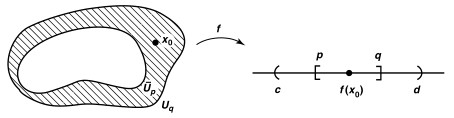
\includegraphics[ width = 0.6\linewidth ]{figures/Section 33/thm33-1.jpg}
            \caption{A visual on the continuity of \( f \)}
            \label{fig:33-2}
        \end{figure}
    \end{proofBox}
\end{thmBox}

\begin{thmBox}{33.2}[thm:33.2]
    A subspace of a completely regular space is completely regular.
    A product of completely regular spaces is completely regular.

    \baseRule

    \begin{proofBox}

    \end{proofBox}
\end{thmBox}